\chapter*{LINUX EN EL GOBIERNO}
Este capítulo se basará en aquellas naciones en las que Linux a pasado a formar parte de su estructura interna. También se explicará las causas que originó este cambio y como 
principal consecuencia, el impacto social que este importante sistema operativo a generado a lo largo del proceso de implementación que adoptaron estos países.

\section*{BRASIL}
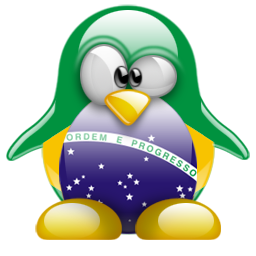
\includegraphics[scale=0.5]{img/cp03/img0301.png}

Tras un largo período en el que Brasil destinaba parte de su presupuesto al pago de licencias de Microsoft y Apple, optó por una alternativa que lo condujo a posicionarse como 
uno de los países pioneros en el uso de software libre. Fue en el gobierno del aún presidente Luiz Inácio Lula da Silva que se inició el cambio de Windows a Linux. La medida fue 
implementada con una gran acogida por parte de la sociedad Brasileña, ya que para la mayoría representaba una alternativa económica importante pensando en los no tan numerosos 
recursos.                                                 
                                                                                                                                  
Con esta puesta en escena que realizó Brasil se han logrado grandes avances en materia de desarrollo tecnológico, además de que se ha creado una cultura del libre desarrollo en 
la sociedad de este potente país, inculcando desde las aulas de clase el uso de dicho software desde muy temprana edad.                                                          
                                                                                                                                  
Brasil, se ha convertido en el principal país no sólo en América sino en el mundo más comprometido en la fomentación de código libre, esto le a permitido grandes ganancias ya que 
ahora no tendrá que invertir en licencias costosas como lo solía hacer con Microsoft y Apple, ahora podrá destinar estos recursos a proyectos de investigación. Con la 
implementación de este sistema operativo, se produjo en el 2008 un considerable ahorro de unos US\$ 167,8 millones de dólares. La empresa encargada de ofrecer dicha solución es 
Userful Corp, esta es una pequeña compañía canadiense encargada de desarrollar la aplicación "Multiplier", esta se ejecuta como un servicio del sistema operativo y permite que un 
computador de mesa sea compartido hasta por 10 usuarios todos conectados. 


\section*{ALEMANIA}
Al igual que Brasil, Alemania y más exactamente la ciudad de Munich que utilizó en sus sistemas de redes y de seguridad el conocido y tradicional sistema operativo de Microsoft 
ahora a optado por cambiarse a Linux, justificando como causa el "desperdicio electrónico" de computadoras con Windows, como consecuencia de esto Munich, (la tercera ciudad más 
importante de Alemania) a destinado 30 millones de euros para tal propósito. Se puede decir que Alemania se perfila entonces a migrar posiblemente en todo su territorio a este 
sistema operativo “Linux”, ya que ademas de la evidente seguridad que este sistema operativo pueda ofrecerle gana también el país en el ámbito económico, por ser este, de 
circulación gratuita.                      
                                                                                                                                  
Para lograr una mayor aceptaciòn por parte de la comunidad alemana, el paìs ofrece gratuitamente a los habitantes de Munich  miles de discos con Linux, así podrán estos comenzar 
a hacer uso del sistema operativo ademas de un acompañamiento que se prestara en diferentes instalaciones tales como colegios y/o universidades.               
                                                                                                                                 
Lubuntu, "un derivado de Ubuntu", fue la distribución por la cual Munich apostó, especialmente por ser gratuito y por los costos no tan altos de memoria y eficiencia energética 
que estaban acostumbrados a gastar con Microsoft; las razones primordiales por las cuales se tuvo en cuenta en la elección de esta versión de sistema operativo fue que Lubuntu no 
presentaba problema con los requisitos de hardware, mientras que por su parte otras distribuciones si, además de la importante similitud en cuanto al entorno gráfico con Windows 
XP.                                                              
                                                                                                                                 
Los expertos en IT(tecnologías de la información) han expresado su voz de inconformismo ya que consideran a Windows un sistema operativo vulnerable y peligroso a la vez pensando 
en lo que pudieran llegar hacer agencias gubernamentales, si éstas tienen acceso a la información confidencial del gobierno Alemán, justificando que Microsoft tiene una 
desventaja en seguridad: su backdoor, la cual es una especie de puerta trasera que seguramente podría favorecer a la NSA (National Security Agency) encargada en las tareas de 
seguridad de la información y espionaje del gobierno estadounidense; la solución a dichos problemas, según estos expertos, es la inmediata migración al sistema de código abierto 
Linux.                           
                                                                                                                                 
La administración pública alemana e IBM(International Business Machines) la cual es una empresa multinacional estadounidense de tecnología y consultoría, suscribirán un acuerdo 
que implica que miles de servidores serán migrados a la plataforma Linux.. Queda pues claro que con el pasar del tiempo y a medida que Linux ofrece un mejor desarrollo y mejoras 
en su sistema, se posiciona como uno de los favoritos en la lista de los sistemas que brindan seguridad, robustez y ademas a un precio muy cómodo para sus usuarios. 


\section*{CUBA}
En Cuba, el acceso a una computadora resulta una tarea bastante complicada, aún más difícil resulta poder conectarse a una red, sin tener en cuenta que este país cuenta con un 
restringido ancho de banda para el acceso a internet, esto debido a la intervención de los Estados Unidos de América en la no posibilidad de tener un mayor acceso a la web por 
parte de los interesados en hacerse a estos servicios; es así pues, como resulta casi imposible el hecho de no solamente adquirir una computadora sino también el navegar en 
alguna de estas, sin antes pasar por una especie de "autorización" por parte del gobierno cubano, de la cual la gran mayoría no salen bien librada.                                                                                                    

Segun Alain Turiño (profesor de proyectos informáticos en escuelas cubanas) "El primer paso para lograr una migración exitosa en un país, es que el proceso educativo en todos sus 
distintos niveles se desarrolle con software libre para que así las industrias tengan un personal calificado cuando comience un proceso de migración en las mismas".                                                 

Está claro pues, que resulta muy conveniente por parte de los países interesados adoptar este tipo de iniciativas a su plan de recontextualización curricular; para así, no solo 
garantizar una familiarización, ni un óptimo manejo de un sistema operativo diferente, sino ademas, estar preparados a los distintos posibles escenarios que se presentan 
diariamente en el mundo laboral.                                                                       
                                                                                                                                 
Es así, como ante la negativa de EE.UU para el uso de Windows de manera accesible desde todos los aspectos en Cuba, el software libre encuentra un espacio para crecer, como una 
forma de defender su soberanía informática, el gobierno cubano a buscado soluciones a estas problemáticas y así no depender de lo que pueda ofrecerle solamente el software 
privativo. 

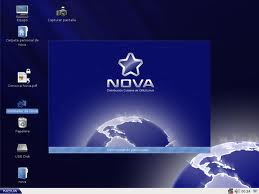
\includegraphics[scale=0.6]{img/cp03/img0302.png}

\textit{" El Software libre está llamado a liderar la lucha de clases en el entorno digital para garantizar la soberanía tecnológica en América Latina"}, afirmó el académico 
Orlando Cárdenas durante la XV (Décimo Quinta)Convención y Feria Internacional Informática 2013, con sede en la capital Cubana.

Se desarrolla entonces Nova, una interesante distribución de GNU/Linux,  creada por estudiantes y profesores de la Universidad de las Ciencias Informáticas de Cuba, teniendo como 
misión facilitar la migración a código abierto. Nova, también fue implementado a causa del bloqueo que impartía EE.UU en el parque tecnológico de Cuba, y vieron a ésta 
distribución como una luz al final del túnel, la esperanza volvía.

El líder del proyecto, Angel Goñi, asegura \textit{"que el sistema permite utilizar aplicaciones modernas en una interfaz sencilla y trabajar con las máquinas obsoletas que 
todavía abundan en la isla, aunque no es "la plataforma" definitiva de Cuba para migrar a Linux"}. Esta distribución, se ha convertido en un tipo de salvavidas para los 
habitantes de la isla, para así poder evadir las restricciones que les fueron implantadas por los EE.UU desde 1962, en las cuales incluye compra de programas y las 
actualizaciones de los mismos.                          
                                               
"Los sistemas de plataforma abierta nos permiten, en la medida que se vayan dominando todas estas técnicas y se siga profundizando en ellas, lograr una mayor inviolabilidad en 
los procesos de informática", dijo a periodistas el comandante Ramiro Valdés Menéndez, exministro del Interior del gobierno cubano.


\section*{CHINA}
Ya se ha mencionado anteriormente que la actual posición de Microsoft se ha visto afectada, pues ha disminuido su uso en países importantes con la llegada de Linux. Para el caso 
de China esto no es diferente pues, hace algún tiempo, Dell quien anunció una posible alianza con Oracle, serían los encargados de ofrecer a China un producto basado en Linux, 
todo con el fin de disminuir el creciente mercado que maneja Microsoft.

Tiempo después que el mundo informático conoció la noticia de que China incurriría en un sistema operativo como Linux para empezar a dejar a un lado el privativo sistema de 
Microsoft, las reacciones de este, no se hicieron esperar e inmediatamente tomó acciones tales como; la creación de versiones de Windows en el idioma nativo de las localidades de 
todo el mundo.

A pesar de estos esfuerzos realizados por Microsoft, pocos años después la versión GNOME de Ubuntu no tardó en llegar para luego ser aceptada oficialmente por parte de la 
comunidad China. "Las empresas Chinas pueden llegar a ahorrarse un 70 por ciento en la compra de un servidor si escogen un servidor Dell con Base de Datos de Oracle basado en 
Linux", afirmó Foo Piau Phang, presidente de Dell en China, en un intento por erosionar la actual posición dominante del sistema operativo de Windows de Microsoft.

Es apenas lógico y natural que Microsoft se inquiete al ver que China quiera empezar grandes cambios en cuanto a seguridad informática se refiere, puesto que este país representa 
la mayor economía del mundo y a Microsoft le traería pérdidas millonarias. Pero es tanto el terreno que ya ha ganado Linux en esta nación, que los academicos de la Universidad 
Nacional de Defensa Tecnológica en la República Popular de China desarrollaron un sistema operativo "Kylin", aprobado para el uso del ejército y la defensa nacional.

Cabe decir que este sistema operativo esta basado en Mach t FreeBSD, lo que le permite un nivel extra de seguridad al sistema operativo, y que es idéntico a (Security-Enhnaced 
Linux, "Seguridad Mejorada de Linux") que fue primeramente desarrollado por la Agencia de Seguridad Nacional de los Estados Unidos.


\section*{MÉXICO}
El gobierno del Distrito Federal de Ciudad de México ha decidido migrar en su administración al sistema operativo de código abierto, Linux; dejando a un lado el uso del software 
privativo Microsoft. Justificando como razón de cambio las innumerables ventajas que éste trae, algunas de ellas son: la independencia, el control de la información, la 
confiabilidad y estabilidad, la seguridad, y el importante ahorro económico.

Independencia: Con la adquisición de Linux, el gobierno es dependiente de sí mismo, ya que no estará en la obligación de rendirle cuentas a un ente extranjero que cerciore su 
manejo interno.

Control de la información: Linux, al ser un sistema operativo de código abierto tiene la posibilidad de ser modificado al antojo de quién lo manipule.

Confiabilidad y estabilidad: Una importante cantidad de personas previamente seleccionadas, están autorizadas de ponerse en la tarea de analizar los errores y buscar soluciones 
óptimas, permitiendo así que el sistema operativo sea confiable y estable.

La seguridad: Sin duda uno de los puntos más importantes para el gobierno, pensando en lo que pueden llegar a hacer países especialmente como EEUU, si éste llegase a tener acceso 
a la información que el país manito maneje, resulta una tarea bastante fácil el desterrar la presencia de puertas traseras y el controlar las posibles filtraciones en 
información; esto gracias al software libre.

Ahorro económico: El pago de actualizaciones y de licencias de programas ya no será más un dolor de cabeza para el estado mexicano, y se podrá destinar este dinero a 
mantenimiento de hardware y capacitaciones para el rápido acoplamiento a Linux.

En el gobierno de la capital mexicana, se puede apreciar un ejemplo vivo de la utilización de software libre y una de sus ganancias, el ámbito económico; cerca de 6000 y 9000 
pesos por cada computadora personal, es uno de los ahorros logrados, gracias a su programa software libre como gobierno GDF/Linux, al evitar la adquisición o actualización de 
licencias, paquetería ofimática(conjuntos de herramientas de administración) y antivirus entre otros, todo por cambiar de un sistema operativo de código abierto a uno cerrado.

Según Ron Hovsepian presidente y jefe de operaciones de Novell (compañía dedicada al software, específicamente en el área de sistemas operativos de redes), afirma que "El código 
abierto significa un nuevo mundo de negocios y opciones técnicas". Por su parte, Fernando Romo, Sandino Araico, José Luis Chiquete y Miguel de Icaza, todos estos importantes 
líderes reconocidos en el ámbito del software libre comentan que "el que utiliza Linux ya no solo es el estudiante de universidad o un programador avanzado sino que a esto, 
empresas de renombre IBM(Mejor conocido como el gigante azul, Gigante Azul, es una empresa que fabrica y comercializa hardware y software), HP(Hewlett-Packard, la cual es una 
empresa de tecnología de la información) y Novell utilizan este sistema operativo en su respectiva infraestructura tecnológica".


\section*{FRANCIA}
Reducir el gasto público, esa es la medida por la cual el gobierno Francés se inclinó para migrar al sistema operativo de código abierto, Linux; esto con el importante apoyo y 
consentimiento de los distintos ministerios de este país. El ministro de función pública ó servicio civil, Renaud Dutreil, dijo a Reuters(agencia de noticias) que 
\textit{" Francia quería que proveedores de software de fuente abierta reabastecieran parte de los casi un millón de ordenadores estatales en virtud de un plan gubernamental de 
reducción de gastos destinado a recortar un abultado déficit público"}

"En juego, sólo en el caso del software de ofimática, están unos 300 millones de euros en programas que serán cargados en ordenadores estatales en tres años. Los ahorros en 
sistemas operativos podrían ser de un orden similar", dijeron responsables oficiales. Cabe mencionar que uno de los factores que incluyó en la migración a Linux fue el afán del 
gobierno francés por minimizar los costos de operación, al mismo tiempo que éste buscaba frenar un déficit en el sector público, el cual muy seguramente le acarrearía problemas 
con la Unión Europea si se superase el 3\% del producto interior bruto, mejor conocido como BIP.

El software de fuente abierta - programas sin derechos de autor que no tiene coste de licencia - como Linux, OpenOffice, Mozilla, Apache, MySQL y Evolution - es "muy creíble", 
dijo Dutreil. Tal fue la acogida por parte del país galo que no demoró mucho tiempo en trasladarse este fenómeno de código abierto a la educación. Red Hat Enterprise, fue la 
distribución elegida por el ministerio de educación francés para la implantación de Linux en las aulas de clase. La decisión fue tomada pensando en liberarse de cierta forma de 
las restricciones y ciclos de actualizaciones  impuestas por software de tecnología propietaria.


"Más de 3.000 servidores, lo que supone entre 80 y 120 servidores por delegación de educación local, ahora operan con Linux, con un 80 por ciento de ellos corriendo sobre Red Hat 
Enterprise Linux", explicó Michel Affre, responsable de sistemas de TI del Ministerio de Educación Francés.

Una decisión estratégica y rentable parece haber sido adoptada en el momento oportuno, aparte del gran recibimiento por parte de los integrantes más jóvenes del departamento de 
TI(Tecnologías de Información) del ministerio. Dejando atrás licencias, contratos de permanencias, restricciones, etc. Sin duda, un grandísimo acierto por parte de Affre.

"En 2004, cerca del 95 por ciento de los servidores corrían sobre Linux. Hoy en día, estamos cerca del 100 por cien, desde que retiramos los últimos servidores AIX a finales de 
2006", añadió Affre. "Gracias a sus servicios de soporte profesionales, Red Hat Enterprise Linux fue la clara elección para nuestros servidores de misión crítica los cuales 
ejecutan los sistemas esenciales de administración para las escuelas de toda Francia".

El fenómeno del software libre parecía no cesar, esta vez la Gendarmería (Policía gala) deja el sistema operativo que venía funcionando desde que ésta existía, el conocido 
Windows. La prensa británica afirma que ésta institución tomó esta medida pensando en los no tan bajos costos de licencia de software privativo. Por su parte la Gendarmería gala 
asegura que este cambio le permitirá un considerable ahorro del 40\% frente al software de código cerrado, manejado por Microsoft. Hasta el momento, 72000 computadores es la 
cantidad que han migrado al software libre en este organismo del estado.


\section*{ECUADOR}
La historia de Linux en Ecuador se remonta a 2006 cuando el presidente electo en ese año, Rafael Correa tuvo una reunión con Richard Stallman, más conocido como el padre del 
software libre. Tiempo después de esta trascendental reunión, Correa le hizo saber al pueblo ecuatoriano la importancia del software libre, y a su vez no dudó en invitar a que 
usaran este software de código abierto.

"Es necesario que todos adoptemos tanto a nivel público y a nivel privado el software libre, de esa manera garantizaremos la soberanía en nuestros estados, dependeremos de 
nuestras propias fuerzas, no de fuerzas externas a la región. Seremos productores de tecnología, no simple consumidores, seremos dueños de los códigos fuentes, y podremos 
desarrollar muchos productos, que incluso con una
adecuada articulación de nuestros esfuerzos pueden ser de suma utilidad para las empresas públicas y privadas de la región. Por eso todos a utilizar software libre, el gobierno 
ecuatoriano ya lo estableció como una política de gobierno y de estado, esto será un importante paso para la integración y por que no decirlo, para la liberación de América 
latina" Sentenció en el marco de FLISOL ( Festival Latinoamericano de Instalación de Software Libre) el en ese tiempo ya presidente de Ecuador.

El Decreto presidencial 1014 del 10 de abril de 2008 decía exactamente:"Establecer como política pública para las Entidades de la Administración Pública Central la utilización 
de Software Libre en sus sistemas y equipamientos informáticos". Lo que en un principio se creyó que solo aplicaría para la rama ejecutiva, terminó expandiéndose aún más y 
llegase tan lejos como no se esperaba.

Sin duda, el momento en el cual el software libre tocaba de lleno las entrañas del poder ejecutivo fue cuando se instaló OpenOffice para acciones netamente ofimáticas. Fue ahí 
cuando se sintió el cambio de software privativo a software libre.

Tiempo después, exactamente en el 2008 fue cuando gracias a un decreto impartido por la asamblea constituyente de este país, es a partir de entonces cuando el poder legislativo 
también utilizaría herramientas similares que el poder ejecutivo.

eCURUL, ha sido uno de los más importantes descubrimientos del software libre en la administración ecuatoriana, éste programa permite no sólo realizar votaciones electrónicas en 
tiempo real sino también controlar debates gubernamentales. Posteriormente, Zimbra, un interesante programa para el control de los correos electrónicos. Sin lugar a dudas, no se 
estaba desperdiciando por parte del gobierno ecuatoriano el grandísimo potencial del sistema operativo de código abierto.
Ecuador ha pensado en todo, tanto es así que se habilitó una página web por parte del gobierno donde las personas interesadas en capacitarse en el software libre lo puedan hacer 
sin ningún costo, logrando así que el miedo a manejar o manipular este tipo de software desaparezca. Donde además se encontrará todo tipo de información relacionada con sistemas 
de tecnología abierta.

Ecuador ha conseguido un importante puesto de admiración en la implantación del software libre en su estado, se convirtió en un ejemplo a seguir para sus países vecinos, De 
hecho, Reynaldo Gaibor(Subdirector de Seguridad Informática del Consejo Nacional de la Judicatura de Ecuador) aseguraba en la conferencia que "aunque de momento, no hay acuerdos 
con otros países, la idea es crearlos".


\section*{COLOMBIA}
Para la coordinadora de comunicaciones externas cámara de comercio de Cali, Yaira Arroyave Monsalve, el software libre en Colombia se está convirtiendo en "Una tendencia en 
expansión",  tanto es así, que no solamente las más de 24 entidades de la administración pública colombiana ya trabajan con sistemas de tecnología de código abierto, sino que 
además muchas de las empresas del sector privado también se han unido a esta interesante alternativa de cambio. Aislando el obligado pago de las licencias de actualización del 
software privado, trayendo consigo los importantes beneficios que acarrea migrar a sistemas basados en software libre.

Alrededor de 250 empresas tanto públicas como privadas han decidido adoptar estos sistemas en su funcionamiento interno. Un ejemplo de esta migración es la empresa prestadora de 
servicios públicos del Valle Emcali, donde la totalidad de sus computadoras operan con software libre, convirtiéndose así en un modelo a seguir en el mundo empresarial
.
\textit{" Los colombianos le están perdiendo el miedo al cambio y han migrado de sus sistemas tradicionales al software libre"} Afirma el ingeniero electrónico Mario Alberto Melo. 
Por su parte para Jessica Perea, asesora comercial de Kazak, empresa experta en Linux y software libre de la capital Vallecaucana, la decisión de implantar software de tecnología 
libre en una determinada organización \textit{"depende especialmente del departamento de sistemas, porque de ser por el área administrativa ya muchas lo estarían aplicando. La 
razón: los costos"}. 

Pensando en costos, las tareas de instalación, capacitación y de mantenimiento de un sistema operativo de cualquier empresa se ahorraría una importante suma de dinero si se 
hablase de software libre en vez de software propietario. Otro importante beneficio según Jessica Perea es que "el software libre es modular y entonces se pueden escoger sólo las 
aplicaciones que se necesitan y armar paquetes personalizados". Llamando la atención de aquellas empresas interesadas en adquirir un número finito de aplicaciones, optimizando 
sus recursos a corto plazo. Lujo que no se puede dar el software privado.

Pymelibre, es el nombre del portafolios de productos y servicios de Kazak; donde los usuarios podrán ingresar vía internet y armar su propio paquete de aplicaciones conociendo en 
tiempo real el precio de todas y cada uno de estas. Herramienta bastante útil por parte de esta empresa, aventandose frente a las demás en el ámbito de la tecnología. 

Tanto ha sido el aceptamiento del software libre en la administración pública del país cafetero, que organizaciones de ente social, como el Departamento Administrativo Nacional 
de Economía Solidaria, Dansocial, han venido adelantando tareas de capacitación en el área de la informática para que las personas que desconocen su uso puedan no sólo entender 
la importancia de su manejo sino también tener la oportunidad de encontrar un trabajo donde se empleen estos conocimientos. En Colombia las cifras son alarmantes, según Abraham 
Rubio Quiroga, subdirector de esta importante compañía, "de cada 100 personas sólo 6 tienen computador y apenas 14 pueden acceder a internet". Números alarmantes.

Dansocial como empresa comprometida con el desarrollo, lanza una interesante estrategia para adquirir un hardware de bajo costo por parte de instituciones del sector educativo y 
personas de bajos ingresos, su precio oscila entre los \$386200 y los \$579300 para que tanto estas personas como instituciones, al ser software libre, lo programen a su gusto y 
necesidad, olvidándose de las restricciones, y pago de actualizaciones que son impuestas por el software propietario.

ACIS, Asociación Colombiana de Ingenieros de Sistemas dio a conocer los resultados de una investigación donde fueron encuestadas diferentes empresas sobre el uso de software 
libre y estos fueron los resultados: el 75\% a tenido la oportunidad de interactuar con dicha tecnología, el 63\% usaba Linux como sistema operativo y el 26\% lo destinaba a 
labores de seguridad. Porcentajes alentadores, si se tiene en cuenta que en un principio se tenía miedo de cambio de sistema operacional. 

Sin embargo el panorama de la "expansión" del software libre en Colombia es alentador más ha sido fácil, "Todavía no se ha llegado a un punto en el que las aplicaciones 
empresariales del software libre operen de manera armónica y confiable con el software tradicional, y mientras no se evolucione en ese campo muchas compañías tendrán temor de dar 
el paso", afirma el ingeniero de sistemas Alberto Camacho. 

Según Rubio, \textit{"El software libre está creando cada vez más fuentes de riqueza en la economía colombiana. Mientras Microsoft vende licencias, la arquitectura del software 
libre está en la venta de servicios y por eso en Colombia se han creado muchas empresas que desarrollan, capacitan y ofrecen mantenimiento a los nuevos usuarios"}, asegura el 
subdirector de Dansocial . Mientras uno está creado para ser negocio, el otro está creado para promover el conocimiento, trayendo consigo indirectamente las oportunidades 
laborales citadas anteriormente. Esto es importante en un país como Colombia donde su tasa de desempleo es del 10,7\%, punto a favor para el software libre. "El software libre es 
una herramienta para frenar la pobreza y generar inclusión social". Abraham Rubio. 


\section*{ARGENTINA}
Hacia el año del 2003 se fundó en  Argentina la Asociación \textbf{Civil SOLAR (Software Libre Argentina)}, fue así como en este país la implementación y el uso del el software 
libre empezó a tener un auge importante.

Poco a poco y con el pasar del tiempo la sociedad Argentina entendió que este cambio en el uso de un sistema operativo diferente era necesario para la nación, entonces, 
instituciones del saber cómo colegios y universidades entre otros, implementaban y enseñaban el software libre, tanto así que en la provincia de Río Negro el parlamento aprobó la 
ley 4747/12 que establece el empleo obligatorio del sistema de software libre en los tres poderes del estado,  entes descentralizados y empresas con participación estatal.

Ahora Compañías y asociaciones importantes en Argentina como la anterior mencionada trabajan en el desarrollo de software libre promoviendo las ventajas tecnológicas, sociales, 
éticas y políticas del mismo. SOLAR por ejemplo, es un punto central de apoyo y colaboración en instituciones del estado tales como INADI (Instituto Nacional contra la 
Discriminación, la Xenofobia y el Racismo), el INTI (Instituto Nacional de Tecnología Industrial) y otras.

Esta asociación civil (SOLAR), como uno de los principales referentes en Argentina, en cuanto al uso y desarrollo de software libre, ha liderado importantes proyectos con el 
propósito de cumplir con sus objetivos, los cuales en forma general y resumida, enmarcan la libertad de pensamiento y expresión en el uso del ya mencionado software libre.

Hace algún tiempo en Argentina se desarrolló una distribución basada en Debian GNU/Linux, que lleva por nombre Huayra, pensada para brindar comodidad al ser de fácil manejo para 
estudiantes y docentes, no sin dejar a un lado por supuesto la seguridad del mismo sistema operativo. Gracias a este sistema operativo se ven entonces beneficiadas las 
poblaciones de los centros educativos de la nación Argentina, puesto que a través de Huayra se puede disfrutar de multitudinarios programas y aplicaciones educativas; importantes 
para el  variado y fácil aprendizaje, sobre todo de los que apenas empiezan a conocer un sistema operativo que ofrece libertades como las de Linux.

La idea principal que encierra este peculiar sistema operativo es la de "conectar igualdad", es decir que absolutamente cualquier persona que desee disfrutar de los beneficios 
que trae Huayra lo pueda hacer de forma libre. Una interesante pregunta que se plantean los desarrolladores de Huayra  es la de ¿Por qué desarrollar un sistema operativo propio 
de conectar igualdad basado en GNU/Linux?, a la cual responden <<\textit{ Los objetivos del Programa Conectar Igualdad no podrían lograrse nunca de no tener autonomía y soberanía 
tecnológica con respecto a los estándares de corporaciones transnacionales. El desarrollo argentino debe seguir su propio camino.}

\textit{ Pero para ellos tampoco es necesario volver a inventar la rueda. Usar GNU/Linux nos permite, como decía Newton sobre el avance del conocimiento, "pararnos sobre los 
hombros de un gigante". En términos de desarrollo local no implica ninguna forma de dependencia, como lo implica en otros sectores de la industria, el recurrir a tecnología 
desarrollada en los países centrales. Por un lado no implica una merma en la riqueza nacional vía drenaje de divisas en concepto de regalías, dividendos o remesa de utilidades. 
Por el otro, no atrofia la capacidad nacional de avanzar en el rubro tan vital para el desarrollo como el de Investigación y Desarrollo (I+D). Más bien al contrario, la estimula. 
De este modo, al utilizar GNU/Linux gozamos de todas las ventajas de "pararse sobre los hombros de un gigante" sin las desventajas que esto acarrea en algunos sectores}>>. En 
palabras textuales de los desarrolladores. 

Así pues vemos en el gobierno Argentino como sistemas operativos basados en arquitecturas diferentes a las privativas y tradicionales, se introducen para brindar nuevas 
alternativas a problemas y necesidades de personas que día tras día añoran un mejor mundo informático.


\section*{ESPAÑA}
La asociación ESLE (Asociación de Empresas de Software de Euskadi) una de las más importantes en España y quizás la más importante en Euskadi a resaltado la forma en la que el 
software libre a venido creciendo en la región y a lo largo de todo el país español. ESLE destaca y dice que la principal causa por la que el país vasco (Euskadi), y en general 
toda España tiende a la implementación y manejo del software libre al igual que en la mayoría de países donde este se utiliza; es por la reducción de costos.

Realmente mantener y costear las licencias de Windows es un gasto considerable para cualquier país, si se tiene en cuenta que estas no son para nada económicas. Esta inversión en 
licencias y otros pagos hechos para el sostenimiento del mismo software se puede invertir para el beneficio de  la comunidad; tales como proyectos de investigación, calidad en la 
educación y otros, pero esto gracias a un sustancial ahorro obtenido al transmutar a sistema operativo (Linux por ejemplo) que requiere de menos inversión económica.

Claro esta que aunque si hay una reducción  de los costos tras la implementación de un diferente sistema operativo, es de igual importancia decir que este cambio tiende cada vez 
más y se propaga a diferentes partes del país gracias a la eficiencia administrativa del software libre, lo anterior es una de las principales conclusiones a que llegó ESLE tras 
el primer observatorio de tendencias que él mismo elabora.

Un ejemplo claro de la importante acogida que a tenido el software libre en España es el hecho de las relevantes distribuciones que han visto su origen en esta nación, se 
presentan a continuación las más importantes:

\subsection*{TRISQUEL (GALICIA)}
Trisquel GNU/Linux es una versión del sistema operativo GNU que utiliza el kernel Linux-libre. Los principales objetivos del proyecto son la producción de un sistema operativo 
totalmente libre, fácil de usar, completo, y con buen soporte de idiomas. Las versiones actuales incluyen traducciones para los idiomas Gallego, Inglés, Español, Catalán, Vasco, 
Chino, Francés, Indio y Portugués.

\subsection*{LLIUREX (VALENCIA)}
Realizada por la Consejería de Educación de la Generalidad Valenciana, su objetivo principal es la introducción de las nuevas tecnologías de la información y la comunicación 
basadas en software libre en el sistema educativo de la Comunitat Valenciana. LliureX está basada en Ubuntu, pero las versiones anteriores estaban basadas en Debian.

Se distribuye en las dos lenguas cooficiales de la Comunidad Valenciana, el valenciano y el castellano, y en dos modalidades: para instalar y como CD autónomo (LiveCD).

\subsection*{MOLINUX (CASTILLA)}

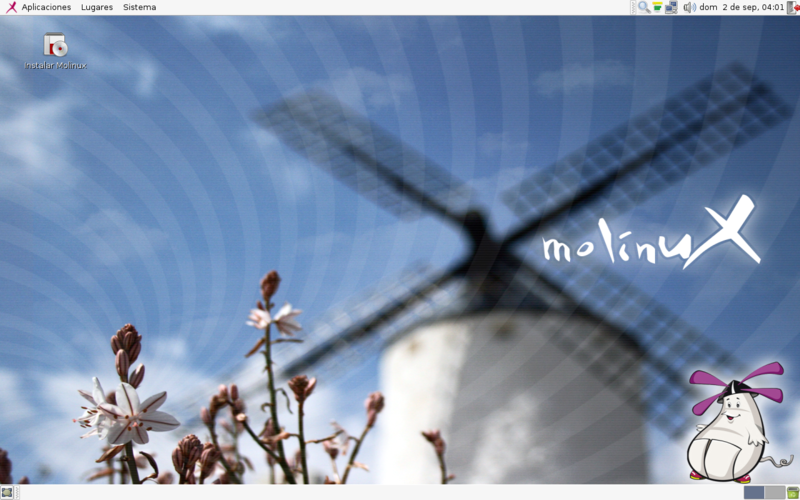
\includegraphics[scale=0.3]{img/cp03/img0303.png}

MoLinux es la distribución GNU/Linux oficial de la Junta de Comunidades de Castilla-La Mancha. MoLinux está basado en Ubuntu. Los nombres de cada versión son personajes de la 
novela "El ingenioso hidalgo don Quijote de la Mancha", de Miguel de Cervantes.

\subsection*{ASTURIX (ASTURIAS)}
Asturix es una distribución GNU/Linux basada en Kubuntu dirigida a usuarios finales y empresas. Es estable, rápida, segura y muy fácil de usar. Consta de varias versiones: 
estándar y lite (para ordenadores con pocos recursos y micro-portátiles).

\subsection*{ASLINUX}
ASLinux Desktop está disponible para CPUs Intel y AMD de 32 bits, posee un entorno completo, estable e intuitivo que facilita el acceso a Linux y que incluye todas las 
características que un usuario final puede exigir: ofimática, Internet, multimedia, educación, juegos, etc., junto con los sistemas de seguridad completos, como un cortafuegos 
personal, un analizador de virus para Windows y un filtro de correo basura. ASLinux Desktop combina la fuerza y estabilidad de Linux, la potencia y versatilidad de Debian Sarge y 
la amigabilidad y facilidad de uso de KDE. Su punto fuerte es su gran usabilidad.


\section*{VENEZUELA}
No se puede terminar este capítulo, sin antes hacer referencia a uno de los gobiernos en los que el software libre predomina con mayor intensidad; más que en muchos otros países, 
incluso de los anteriormente mencionados .

Un hecho que ratifica lo dicho, es el Congreso Nacional de Software Libre (CNSL), que tiene lugar en este país desde el año 2005. El CNSL es un evento de integración social más 
que un evento tecnológico, el objetivo principal es promover la libertad del software, reforzar los valores primordiales de la sociedad, promover independencia tecnológica, la 
producción nacional y la soberanía, y que las personas sepan del significado real del mismo, así como también el de su filosofía. 

Existe en Venezuela una organización (GLoVE), encargada de liderar los congresos Nacionales llevados a cabo este país, para esta organización, lo mas importante para lograr un 
potencial desarrollo del software libre, es la inclusión social en todas sus formas de expresión. Como muchas veces a enfatizado uno de los fundadores del proyecto Octavio 
Rossell "el CNSL es un medio más que un fin".

\textit{"Muchos usuarios y usuarias en el mundo no conocen el término de Software Libre, porque empresas, políticos y medios de comunicación en el mundo lo llaman Código 
Abierto, con el propósito de confundirlos"}, dijo Richard Stallman, es tal vez esta, una de las razones por las cuales, a pesar de que día tras día el uso del software libre, en 
distintos países a crecido, no es lo suficientemente bien conocido por las personas.
